\section{Bilag til beregning af forforstærker}

Dette bilag vil forklare på hvilken måde et Common emitter trin med uafkoblet emittermodstand beregnes. Et sådan kredsløb er vist på figur \ref{fig:commonemitter}

\begin{figure}[h]
\centering
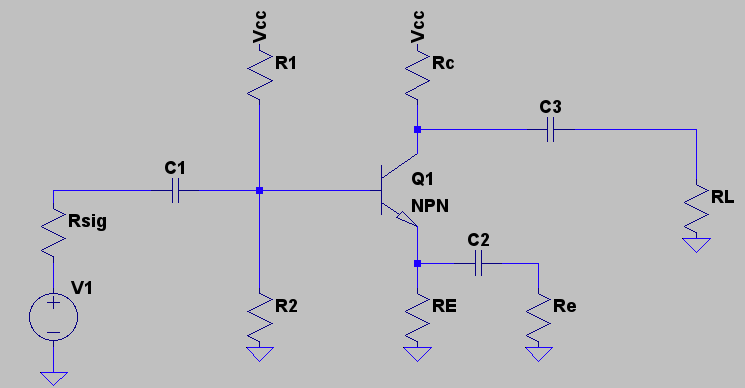
\includegraphics[scale=.6]{teknisk/forforstaerker/bilag/commonemitterfigur.png}
\caption{Common emitter forstærker med uafkoblet emittermodstand}
\label{fig:commonemitter}
\end{figure}

Den maksimale collectormodstand ($R_c$) beregnes ud fra at trinnet skal have så stor en råforstærkning som muligt. Grunden til at der stræbes efter stor råforstærkning er at have så meget som muligt at kunne tilbagekoble for derved at sænke THD. Den maksimale $R_c$ er givet ved ligning \ref{eq:rcmaks}.

\begin{equation}
R_c = \sqrt{\frac{ V_{R_c} \cdot R_{sig} \cdot R_L } { h_{FE} \cdot V_t}}
\label{eq:rcmaks}
\end{equation}

$V_t$ er en konstant, hvis værdi er $26 \cdot 10^{-3}$, $h_{FE}$ er aflæst til 250. $R_L$ og $R_sig$ er afhængig af hvilket trin der beregnes. $V_{R_c}$ er bestemt ud fra ligning \ref{eq:vrcberegning}

\begin{equation}
V_{R_c} = V_{CC} - V_{CE,sat} - V_{R_E} - V_{out,peak}
\label{eq:vrcberegning}
\end{equation}
 
$V_{CE,sat}$ er aflæst til 0,2 V, $V_CC$ er valgt til 15 V og $V_{out,peak}$ er afhængig af hvilket trin der beregnes eftersom amplituden på signalet vil stige efter hvert trin.






$R_L$ og $R_{sig}$ er afhængig af hvilket trin der beregnes på. 